%!TEX root = ../main.tex
\documentclass[a4paper,oneside,12pt, class=Latex/Classes/PhDthesisPSnPDF, crop=false]{standalone}
\usepackage{setspace}
\begin{document}
\doublespacing
\chapter{Introduction}
\label{chap:intro}

\section{The final stages of stars}

\begin{figure}
    \centering
    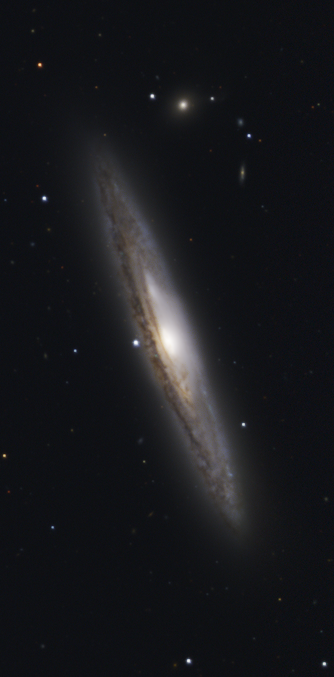
\includegraphics[width=0.49\textwidth]{../Images/chapter_1/SN2024gy_pre-SN.png}
    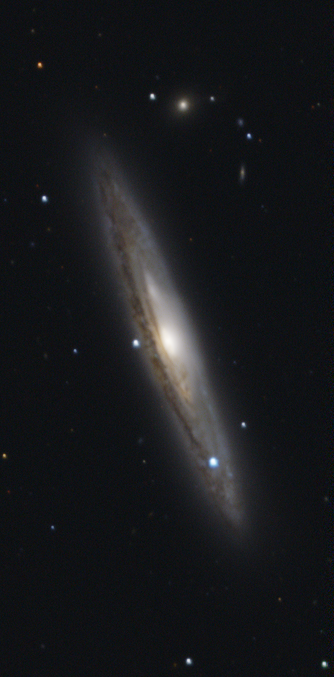
\includegraphics[width=0.49\textwidth]{../Images/chapter_1/SN2024gy_active.png}
    \caption{\ztfg\ztfr\ztfi\ composite image of NGC4216 using observations taken by the Zwicky Transient Facility. \textbf{Left:} composite image of observations taken before 1 January 2024. \textbf{Right:} composite image of observations taken between 5 and 19 January 2024, the first two weeks after the first detection of the Type Ia SN~2024gy. (Credit: Benjamin Nobre Hauptmann) \color{red}Use this as an example when introducing transients \color{black}} %30, 29, 14 (gri sn images) & 35, 31, 30 (gri pre-SN images) given to Benjamin, all used or a subset? --> subset used based on data quality, exact numbersnot so relevant
    \label{2024gy_ZTF}
\end{figure}

\section{Type Ia SNe}
\color{red}Somewhere state that while I focus on interaction in SNe Ia, this search can be broadened, as is done in paper II \color{black}

To convert between apparent and absolute magnitude I assume a flat $\Lambda$CDM cosmology with H$_0 = 67.7$ km s$^{-1}$ Mpc$^{-1}$ and $\Omega_\text{m} = 0.310$ \citep{Planck18VI} throughout this paper, unless specified otherwise. \color{red} Do I use another one anywhere? \color{black}

\end{document}